\documentclass[runningheads]{llncs}

\usepackage{graphicx}
\usepackage{todonotes}
\usepackage{listingsutf8}
\usepackage[hidelinks]{hyperref}
\usepackage{cleveref}

\renewcommand\UrlFont{\color{blue}\rmfamily}

\begin{document}

\title{GeoSPARQL 1.1: an almost decadal update to the most important geospatial LOD standard}
\titlerunning{GeoSPARQL 1.1}

\author{
    Nicholas J. Car\inst{1}\orcidID{0000-0002-8742-7730} \and \\
    Timo Homburg\inst{2}\orcidID{0000-0002-9499-5840} \and \\
    Simon J.D Cox\inst{3}\orcidID{0000-0002-3884-3420}
}

\authorrunning{Car N.J. et al.}

\institute{
    {
    SURROUND Australia Pty Ltd., Australia \&\\
    Australian National University, Australia\\
    \email{nicholas.car@surroundaustralia.com}\\
    \url{https://surroundaustralia.com}
    }
    \and
    {
        Mainz University Of Applied Sciences, Germany\\
        \email{timo.homburg@hs-mainz.de}
    }
    \and 
    {
        Commonwealth Scientific \& Industrial Research Organisation, Australia\\
        \email{simon.cox@csiro.au}
    }
}

\maketitle

\begin{abstract}
The Open Geospatial Consortium published the GeoSPARQL 1.0 standard in 2012 containing multiple 
parts that define ``SPARQL extension functions'', ``RIF rules'', ``an RDF/OWL ontology for 
information based on the General Feature Model'' and supporting vocabularies, all for Semantic 
Web spatial data.\\

In the 8+ years since its publication, GeoSPARQL has become the most important spatial Semantic 
Web standard, as judged by references to it in other Semantic Web standards and its wide use in 
Semantic Web data.\\

An update to the standard was proposed in 2019 to deliver GeoSPARQL 1.1 in 2021 with a charter to: 
handle outstanding change requests and source new ones from the GeoSPARQL user community as well 
to ``better present'' the standard, that is to better link all the standard’s parts and better 
document \& exemplify elements. Expected updates included possible alignments to other ontologies, 
possible handling of new spatial referencing systems, new geometry representations, and new artifact 
presentation.\\

In this paper, we will discuss the submitted change requests and resulting updates to the standard. 
We will also discuss the theory behind updates and our expectations for GeoSPARQL 1.1's use.

\keywords{GeoSPARQL  \and GeoSPARQL 1.1 \and spatial \and geospatial \and Semantic Web \and RDF \and OWL \and OGC \and Open Geospatial Consortuim \and standard.}
\end{abstract}

\section{Introduction}\label{sec:introduction}
The GeoSPARQL standard, first issues in 2021 by the Open Geospatial Consortium (OGC)\footnote{\url{https://www.ogc.org}} 
is one of, if not the most\footnote{It's hard to calculate use but references to GeoSPARQL other well-known standards, 
such as DCAT2 (\url{https://www.w3.org/TR/vocab-dcat/}) suggests this}, used \textit{Sematic Web} ontologies for 
representing spatial data.

The original GeoSPARQL release, which we refere to as GeoSPARQL 1.0, contained a \textit{specification} document,
a main ``GeoSPARQL'' ontology in an RDF file and a ``Simple Features Vocabulary'' ontology also in an RDF file. The 
``GeoSPARQL'' ontology content, as well as lists of geospatial functions that could be performed on RDF data via 
SPARQL\footnote{\url{https://www.w3.org/TR/sparql11-query/}} queries was defined in the specification document, as
were entailement rules and requirements \& abstract tests for testing ontology data and function implementations. 
Within the last few years, the function lists from the sepecification were extracted into a SKOS\footnote{\url{https://www.w3.org/TR/skos-reference/}}
vocabulary.


\section{Motivation to update GeoSPARQL}\label{sec:motivation}
Interest in updating GeoSPARQL had been captured\footnote{\url{https://www.w3.org/2015/spatial/wiki/Further_development_of_GeoSPARQL}}
 by the World Wide Web Consortium's (W3C) \textit{Spatial Data On The Web Working Group} (SDWWG)
when a large body of work was done on \textit{Semantic Web} spatial data around in approximately 2015 - 2017, but 
no updates to GeoSPARQL were ultimately made by that Working Group.

% Spatial Data On The Web Best Practices \cite{van2019best}

Recently, 2019, the OGC reconstituted a \textit{GeoSPARQL Standards Working Group} (SWG) to update GeoSPARQL. The general 
motivation for work within the area of GeoSPARQL, that of \textit{Semantic Web} spatial data, and a series of
fault fixes and proposed extensions to GeoSPARQL 1.0 are captured in an OGC White Paper \cite{geosparqlwhitepaper}. Some,
but not all, of the SDWWG's proposals are included in the White Paper with the different communities - W3C and OGC - 
naturally reflecting different desires.

The SWG's charter - it's final scope of work - is also published by the OGC \cite{abhayaratna2020ogc} and this guides 
the SWG's activities. Specific actions of the SWG and their staging are explained through the use of a publicly-available 
online task tracking system within the SWG's working online code repository\footnote{\url{https://github.com/opengeospatial/ogc-geosparql/projects/1}}.

At a high-level, proposed updates to GeoSPARQL by both the SDWWG and the SWG may be categorised as one of the following:

\begin{itemize}
    \item[$\ast$] new geometry serializations
    \begin{itemize}
        \item[$-$] GeoJSON and other formats that have become popular since GeoSPARQL 1.0 's publication
    \end{itemize} 
    \item[$\ast$] new ontology classes to cater for more nuanced spatial information
    \item[$\ast$] more spatial functions
    \begin{itemize}
        \item[$-$] implementing functions well-known in non \texttt{Semantic Web} spatial systems
    \end{itemize} 
    \item[$\ast$] scalar spatial properties 
    \begin{itemize}
        \item[$-$] area, volume etc. alongside geometries
    \end{itemize} 
    \item[$\ast$] better handling of Spatial (Coordinate) Reference Systems (SRS)
    \begin{itemize}
        \item[$-$] potentially allowing for automated coordinate serialization conversions
    \end{itemize} 
    \item[$\ast$] Internet protocol-based selection of different geometries for features
\end{itemize}

Some of these propsed updates were predicted in GeoSPARQL 1.0 with the \textit{Future Work} section listing several of the 
points above as expected or potential.

The SWG's \textit{Charter}, anticipating that the more obvious updates such as new geometry serializations would certainly
be implemented, listed the following areas of investigation that emerged from SWG proponent's discussions:

\begin{itemize}
    \item[$\ast$] a revision of the ``upper  ontology'' structuring of GeoSPARQL
    \begin{itemize}
        \item[$-$] better/differently defining how GeoSPARQL's \texttt{Feature} and other classes relate to one another and to other fundamental concepts in ontology
    \end{itemize} 
    \item[$\ast$] possible alignments to other ontologies, perhaps the \textit{W3C Time Ontology in OWL}\cite{simon_cox_time_2017}
    \item[$\ast$] catering for new and very different SRSes, such as Discrete Global Grid Systems (DGGS) 
\end{itemize}

Specifically ruled out of scope was any investigation of property graphs. Recent (last several years) discussion in the OGC and 
elsewere about property graphs moticated a consideration of them, hoever the SWG proponents felt that while property graphs might 
be important for future \textit{Semantic Web} spatial data systems, there was more than enough work scoped for initial SWG work
(several revisions of the standard) to initially exclude this are of investigation.

After initial meetings, the SWG determined to make multiple releases of GeoSPARQL updates with different goals:

\begin{itemize}
    \item[$\ast$] \textbf{1.1}: extensions that are fully compatable with GeoSPARQL 1.0
    \item[$\ast$] \textbf{1.2}: fully or mostly compatable extensions but which are larger additions to the standard's conceptual coverage
    \item[$\ast$] \textbf{2.0}: a future GeoSPARQL that might be quite different and partly incompatable with GeoSPARQL 1.0
\end{itemize} 

The reason for expecting a future, incompatable, GeoSPARQL 2.0 is that early SWG attendees thought spatio-temporal relations
and fundamental ontology elements in GeoSPARQL either could or should be remodelled which might break the current, familiar, 
\texttt{Feature}/\texttt{Geometry} class relations. Details of these potential changes haven't been fully expounded, at the 
time of this paper, however initial SWG attendees' intuition is that a future GeoSPARQL 2.0 might generalise spatial concepts and
move away from only, or primarily, \textit{geo}spatial, or perhaps focus not just on \texttt{Feature}/\texttt{Geometry} relations
but look to generalised mechanisms for describing dimensions of features of which \textit{geometry} is one of many (and perhaps)
\textit{temporality} too).

An additional area of updates to GeoSPARQL that was not forseen by GeoSPARQL 1.0, the SDWWG or the initial proponants of the SWG
but which was included by the early SWG attendees in GeosPARQL 1.1 and is now present in the SWG's working repository was that 
of new modes of standard presentation. The motivation for this was conceptual work within the W3C and the OGC to do with how 
multi-part standards might link their parts and declare dependencies. This resulted in the profile declaration work, explained 
in the next section.


\section{Updates in GeoSPARQL 1.1}\label{sec:newfeatures}
So far (as of June, 2020) the GeoSPARQL SWG has triarged changed requests into GeoSPARQL 1.1, 1.2 \$ 2.0 releases and has addressed
many 1.1 requests. Here we report only on those 1.1 requests. This section describes some of the areas updated in GeoSAPRQL 1.1
and the following section foreshadows likely 1.2 and 2.0 updates.

\subsection{Profile Declaration}\label{sec:profiledec}
One of the first actions undertaken by the SWG was to link the GeoSPARQL 1.0 elements through a \textit{profile} 
declaration, where a profile is a special type of \textit{specification}, as defined by \textit{The Profiles Vocabulary}\cite{atkinson_profiles_2020}. 
The specific motivation for this was the SWG's recognition that GeoSPARQL 1.0 consisted of multiple parts, not all
of which were easy to discover and, as a result, some GeoSPARQL users were unaware of some of the resources and some
resources were accidentally duplicated or partly re-implemented. Profile declarations of this sort are anticipated, by the OGC, 
as being the \textit{best practice} way for it to deliver multi-part standards.

The profile declaration for GeosPARQL 1.0 will be published by the OGC as a stand-alone resource sometime in early 2021 along with some 
updated GeoSPARQL 1.0 resources. Currently, all of the elements of GeoSPARQL 1.0, including the profile declaration, 
can be found within the SWG's working online repository \footnote{\url{https://github.com/opengeospatial/ogc-geosparql}}.
The profile declaration for GeosPARQL 1.1 will be published at the same time as all, or most, of the 1.1 releases' updated
resources, currently expected in mid-2021.

\subsection{New geometry literals}\label{sec:newliterals}
GeoSPARQL 1.1 introduces three new litergeometry serializations: 

\begin{enumerate}
    \item GeoJSON (Geo- JavaScript Object Notation)\cite{butler2016geojson}
    \item KML (Keyhole Markup Language)\cite{nolan2014keyhole} 
    \item DGGS (Discrete Global Grid System)\cite{sahr1998discrete}
\end{enumerate} 

The first two of these are ``obvious'' in the sence that that they have been expected/requested by the SDWWG and many users
of GeoSPARQL for a long time, due to those format's popularity. an example of a GeoJSON geometry serialization is given below.

\small
\begin{lstlisting}[caption=GeoJSON geometry serialization example,label=lst:geojsonliteral,language=sql,frame=single,basicstyle=\ttfamily]
"""{"type":"Point", "coordinates":[-83.38,33.95]}"""
^^<http://www.opengis.net/ont/geosparql#geoJSONLiteral>
\end{lstlisting}
\normalsize
Since the GeoJSON and KML formats are restricted to be represented in the WGS84 SRS only, these restrictions 
also apply to GeoJSON and KML literals. The DGGS WKT literal  


The third new serialization format is more forward-looking in that it is not dirven by user demand but by predected demand.
DGGS does not have a single, concrete format standard as the others do, not is it ever likely to - different DGGSes will 
likely implement very different data formats - so GeoSAPRQL 1.1 makes generalized provisions for DGGS serializations but 
presents no detailed requirements for them, only stating that the specific DGGS must be identified.

\subsection{New spatial functions}\label{sec:newfunctions}
GeoSPARQL 1.1 includes new spatial aggregate functions, which allow for the quick aggregation of different geometry types. 
While spatial aggregate functions are the norm in many non-semantic geospatial databases such as POSTGIS or Oracle Spatial, 
at the time of defining the GeoSPARQL 1.0 standard, aggregate functions had not yet been introduced into the SPARQL standard 
since SPARQL 1.1 \cite{w3c_sparql_working_group_sparql_2013} was released about one year later. Spatial aggregate functions 
similar to traditional aggregate functions such as AVG,MAX, or MIN allow to aggregate results of geometry queries, e.g., to 
create the union out of a set of given geometry literal results. While calculating these aggregates may also be possible 
outside of the semantic database, the inclusion of the functions provides distinct advantages:

\begin{enumerate}
    \item No client-side library is needed to create an aggregated geometry result
    \item Fewer and more appropriate results can be returned using a spatial aggregate function (e.g., a single union geometry vs. a set of geometries for which to create union externally)
    \item Spatial aggregates from different SPARQL endpoints can easily be calculated using federated queries 
\end{enumerate}

GeoSPARQL 1.1 defines the aggregate functions \emph{geosf:boundingCircle}, calculating a bounding circle around a set of 
geometry, \emph{geosf:centroid} calculating the centroid of the set of geometries, \emph{geosf:concatLines} concatenating 
a set of linestrings that overlap, \emph{geosf:concaveHull} calculating the concave hull of a set of geometries and\emph{geosf:union}, 
calculating the union of a set of geometreis, in addition to the \emph{geosf:envelope} and \emph{geosf:convexHull} functions 
already defined in the GeoSPARQL 1.0 standard. Since SPARQL 1.1 these fucntions were also usable as aggregate functions.

Spatial aggregate function definitions are accompanied by the functions \href{http://www.opengis.net/def/function/geosparql/maxX}{\emph{geof:maxX}}, 
\href{http://www.opengis.net/def/function/geosparql/maxY}{\emph{geof:maxY}}, \href{http://www.opengis.net/def/function/geosparql/maxZ}{\emph{geof:maxZ}} 
and \href{http://www.opengis.net/def/function/geosparql/minX}{\emph{geof:minX}}, \href{http://www.opengis.net/def/function/geosparql/minY}{\emph{geof:minY}}, 
\href{http://www.opengis.net/def/function/geosparql/minZ}{\emph{geof:minZ}} which allow to retrieve the minimum and maximum 
coordinates of a geometry respectively.

\subsection{Ontology extensions}\label{sec:ontexts}
GeoSPARQL 1.1 extends the GeoSPARQL ontology by adding a new class \href{http://www.opengis.net/ont/geosparql#SpatialMeasure}{geo:SpatialMeasure}. 
This class represents a measurement such as a volume, length, or area associated with a measurement amount and a measurement 
unit. It acts as a range of three newly defined properties \href{http://www.opengis.net/ont/geosparql#hasVolume}{geo:hasArea}, 
\href{http://www.opengis.net/ont/geosparql#hasLength}{geo:hasLength}, \href{http://www.opengis.net/ont/geosparql#hasVolume}{geo:hasVolume} 
which make these attributes of a geometry better accessible using SPARQL. Finally, GeoSPARQL 1.1 adds the 
\href{http://www.opengis.net/ont/geosparql#inSRS}{geo:inSRS} property, which allows querying the SRS of a given geometry 
without the need to analyze geometry literal serializations. The property allows for the definition of a SRS as a URI. It 
paves the way for a future definition of SRS fully in RDF as anticipated for GeoSPARQL 2.0.

\begin{figure}[htb]
    \centering
    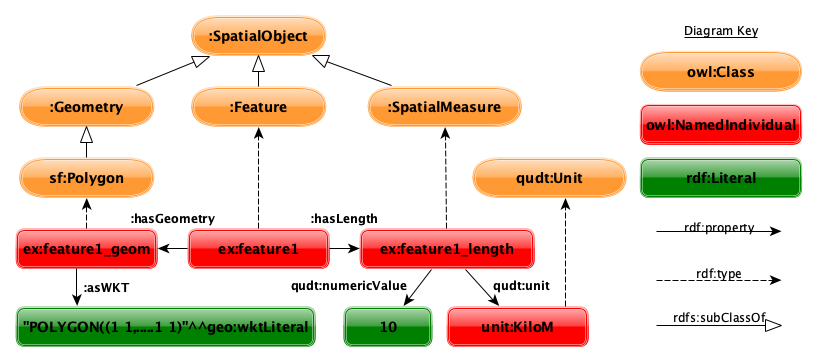
\includegraphics[width=\linewidth]{images/geold_ontology.png}
    \caption{GeoSPARQL 1.1 ontology including one example feature}
    \label{fig:geosparql11ontology}
\end{figure}


\section{Modernizing the documentation of GeoSPARQL}\label{sec:documentation}


\subsection{Profile}\label{sec:profile}


\section{Conclusions}\label{sec:conclusions}

\subsection{Future Work}\label{sec:futurework}
GeoSPARQL 1.2, GeoSPARQL 2.0?
\begin{itemize}
    \item GeoSPARQL extension ontologies: SRS systems
    \item GeoSPARQL 1.2: More literals?
    \item GeoSPARQL 2.0: Full featured support for 3D, simple features functions, coverages?
\end{itemize}
%   History of GeoSPARWL 1.0
% Section 2
%   motivation to update the spec
% Section 3
%   GeoSPARQL 1.1 additions
%       motivation, and expected use, of new spatial functions. In particular, why in GeoSPARQL when aggregations etc. can be performed elsewhere?
%       Spatial Measure
% Section 4
%       new profile preentation
%       new URI regimes etc
% Section 5
%       expected changed use modes


%
% ---- Bibliography ----
%
% BibTeX users should specify bibliography style 'splncs04'.
% References will then be sorted and formatted in the correct style.
%
\bibliographystyle{splncs04}
\bibliography{GeoSPARQL}
%
% \begin{thebibliography}{8}
% \bibitem{ref_article1}
% Author, F.: Article title. Journal \textbf{2}(5), 99--110 (2016)

% \bibitem{ref_lncs1}
% Author, F., Author, S.: Title of a proceedings paper. In: Editor,
% F., Editor, S. (eds.) CONFERENCE 2016, LNCS, vol. 9999, pp. 1--13.
% Springer, Heidelberg (2016). \doi{10.10007/1234567890}

% \bibitem{ref_book1}
% Author, F., Author, S., Author, T.: Book title. 2nd edn. Publisher,
% Location (1999)

% \bibitem{ref_proc1}
% Author, A.-B.: Contribution title. In: 9th International Proceedings
% on Proceedings, pp. 1--2. Publisher, Location (2010)

% \bibitem{ref_url1}
% LNCS Homepage, \url{http://www.springer.com/lncs}. Last accessed 4
% Oct 2017
% \end{thebibliography}
\end{document}




% Outline
% 
% Section 1
%   History of GeoSPARWL 1.0
% Section 2
%   motivation to update the spec
% Section 3
%   GeoSPARQL 1.1 additions
%       motivation, and expected use, of new spatial functions. In particular, why in GeoSPARQL when aggregations etc. can be performed elsewhere?
%       Spatial Measure
% Section 4
%       new profile preentation
%       new URI regimes etc
% Section 5
%       expected changed use modes